\section{Experimental Setup}

Main question to answer, can pre-training on temporal order verification aid action recognition from raw RGB inputs without explicit calculation of optical flow.

Processing video data yields difficulties not present in processing image data.

A single input is higher dimensional (here by a factor of 16).

Input sizes are bigger, therefore only smaller batch sizes possible.

Dataset sizes are too big for fitting into main memory of most common computers.

To distribute video, they are encoded.
To access individual frames, they need to be decoded which increases data sizes further.

Because of memory limitations, creation of a single input batch requires decoding of the involved videos.
Cannot be kept in RAM, so need to be decoded for each new input batch.

Therefore special input pipeline necessary.

\subsection{Hardware Setup}


\subsection{Model Architecture}

Our implementation of the \textit{C3D} model follows the architectural design of the original \textit{C3D} network, as described in \cite{tran_learning_2015} and in the published Caffe implementation (see \mbox{\url{https://github.com/facebook/C3D}}).
We implemented our model in Python using Google's deep learning framework \textit{Tensorflow} \cite{abadi_tensorflow:_2016}.
The \textit{C3D} network contains eight 3D convolutional layers, with max-pooling layers after the first, second, fourth, sixth and eighth layer.
An illustration of the network model is given in figure \ref{fig:c3d_architecture}.
After the last pooling layer, the temporal information is fully collapsed and the feature maps two-dimensional.
These are then flattened into a one-dimensional vector to be further processed by the fully-connected layers.

\begin{figure}[H]
    \centering
    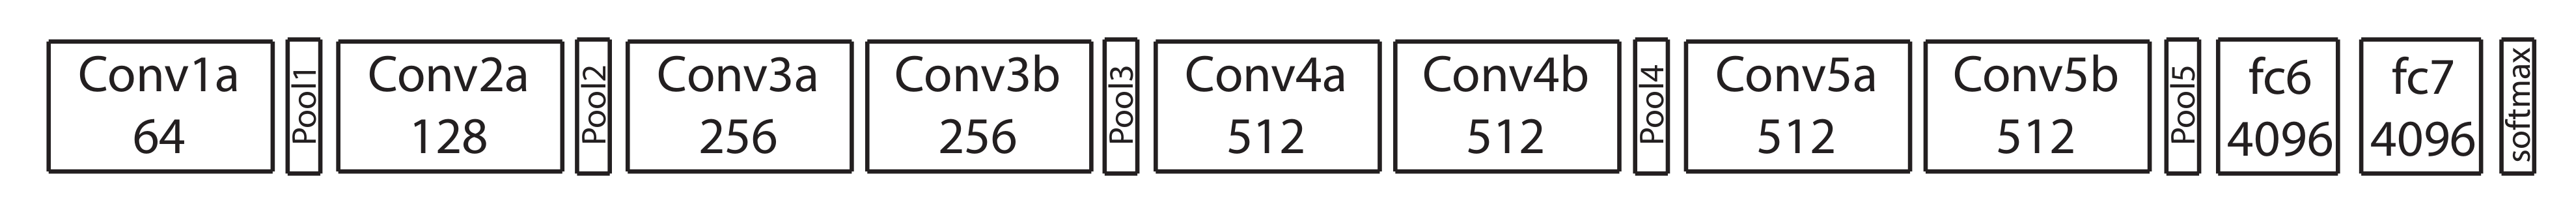
\includegraphics[width=\textwidth]{img_related/c3d_architecture}
    \caption{Illustration of the C3D architecture. An additional flattening operation is performed after \textit{Pool5}, which is not illustrated in this figure. \cite{tran_learning_2015}}
    \label{fig:c3d_architecture}
\end{figure}

\subsubsection{Architectural Details}

According to the experiments conducted by \textcite{tran_learning_2015}, 3D convolutional kernels of size $3 \times 3 \times 3$ perform best in the \textit{C3D} model.
We therefore follow this design decision in our implementation as well.
The network processes inputs of spatial dimension $112 \times 112$ pixels and temporal length of $16$ frames in $3$ RGB channels.
The dimension of a complete input volume therefore is $16 \times 112 \times 112 \times 3$.
The 3D filters in the convolutional layers \textit{conv1a} - \textit{conv5b} are applied to their inputs with stride 1 and zero-padding is applied.
The convolutional layers therefore do not reduce the dimensionality of the inputs in neither spatial nor temporal dimension.

All pooling layers, except the first one, perform $2 \times 2 \times 2$ (\textit{width $\times$ height $\times$ temporal depth}) 3D max-pooling with strides two.
The pooling layers thereby reduce the spatial and temporal dimension of an input by $2$.
The first pooling layer only performs spatial pooling, i.e. with a pooling kernel of dimension $2 \times 2 \times 1$, in order to not collapse the temporal information too early as done in \cite{tran_learning_2015}.
Table \ref{tab:num_params} holds the output dimensions of each layer along with the number of trainable weights and biases.

\begin{table}[H]
    \renewcommand{\arraystretch}{1.3}
    \begin{tabularx}{\textwidth}{l X l}
    Layer Name & Output Dimension & Trainable Parameters \\
    \hline
    \textbf{Conv1a} & $16 \times 112 \times 112 \times 64$ & $3 \cdot 3 \cdot 3 \cdot 3 \cdot 64 + 64 = 5,248$\\
    \textbf{Pool1} & $16 \times 112 \times 112 \times 64$ & 0 \\
    \textbf{Conv2a} & $16 \times 56 \times 56 \times 128$ & $64 \cdot 3 \cdot 3 \cdot 3 \cdot 128 + 128 = 221,312$\\
    \textbf{Pool2}& $8 \times 28 \times 28 \times 128$ & 0 \\
    \textbf{Conv3a} & $8 \times 28 \times 28 \times 256$ & $128 \cdot 3 \cdot 3 \cdot 3 \cdot 256 + 256 = 884,992$ \\
    \textbf{Pool3} & $4 \times 14 \times 14 \times 256$ & 0 \\
    \textbf{Conv4a} & $4 \times 14 \times 14 \times 512$ & $256 \cdot 3 \cdot 3 \cdot 3 \cdot 512 + 512 = 3,539,456$ \\
    \textbf{Conv4b} & $4 \times 14 \times 14 \times 512$ & $512 \cdot 3 \cdot 3 \cdot 3 \cdot 512 + 512 = 7,078,400$ \\
    \textbf{Pool4} & $2 \times 7 \times 7 \times 512$ & 0 \\
    \textbf{Conv5a} & $2 \times 7 \times 7 \times 512$ & $512 \cdot 3 \cdot 3 \cdot 3 \cdot 512 + 512 = 7,078,400$ \\
    \textbf{Conv5b} & $2 \times 7 \times 7 \times 512$ & $512 \cdot 3 \cdot 3 \cdot 3 \cdot 512 + 512 = 7,078,400$ \\
    \textbf{Pool5} & $1 \times 4 \times 4 \times 512$ & 0 \\
    \textbf{Flattening Layer} & 8192 & 0 \\
    \textbf{fc6}& $4096$ & $8192 \cdot 4096 + 4096 = 33,558,528$ \\
    \textbf{fc7} & $4096$ & $4096 \cdot 4096 + 4096 = 16,781,312$ \\
    \textbf{softmax} & \#classes in dataset & $4096 \cdot \text{\#classes} + \text{\#classes}$ \\
    \end{tabularx}
    \caption{Output dimension and number of trainable parameters per layer in our \textit{C3D} model. The flattening layer collapses the feature maps in \textbf{pool5} into a one dimensional vector.}
    \label{tab:num_params}
\end{table}

The total number of parameters in the network adds up to $77,995,776$ plus the parameters residing in the last softmax output layer, whose amount depends on the number of output classes in the used dataset.
We report final results on the UCF-101 and Charades dataset.
The number of total parameters for these datasets are given in the following table \ref{tab:parameters_per_dataset}:
\begin{table}[H]
    \centering
    \begin{tabularx}{\textwidth}{l c c c} 
            Dataset & \#classes & \#Parameters (last layer) & \#Parameters (total) \\ 
            \hline
            UCF-101 & 101 & \hspace{0.5cm} $4096 \cdot 101 + 101 = 413,797$ \hspace{0.5cm} & $\textbf{78,409,573}$ \\
            Charades & 157 & $4096 \cdot 157 + 157 = 643,229$ & $\textbf{78,639,005}$ \\
    \end{tabularx}
    \caption{Total number of parameters in our implemented \textit{C3D} model according to the number of classes in the target dataset.}
    \label{tab:parameters_per_dataset}
\end{table}

As can be seen in table \ref{tab:parameters_per_dataset}, the number of total parameters is two orders of $10$ bigger than the number of parameters in the output layer.
It can be concluded, that most of the networks parameters, namely around $64\%$ are located in the last two fully-connected layers.
This is illustrated in figure \ref{fig:parameters_plot} and common in architectures with fully-connected layers, as they naturally contain more parameters than convolutional layers.
In recent image classification approaches with CNNs ??, the number of parameters is heavily reduces by substituting last fully connected layers.
We address this in section \ref{sec:future_work}.
We keep the architecture unchanged in order to compare our results, more precisely the effect of \textit{temporal order verification} on 3D convolutional networks, to the results of \textcite{tran_learning_2015} and \textcite{carreira_quo_2017}.

\begin{figure}[H]
    \centering
    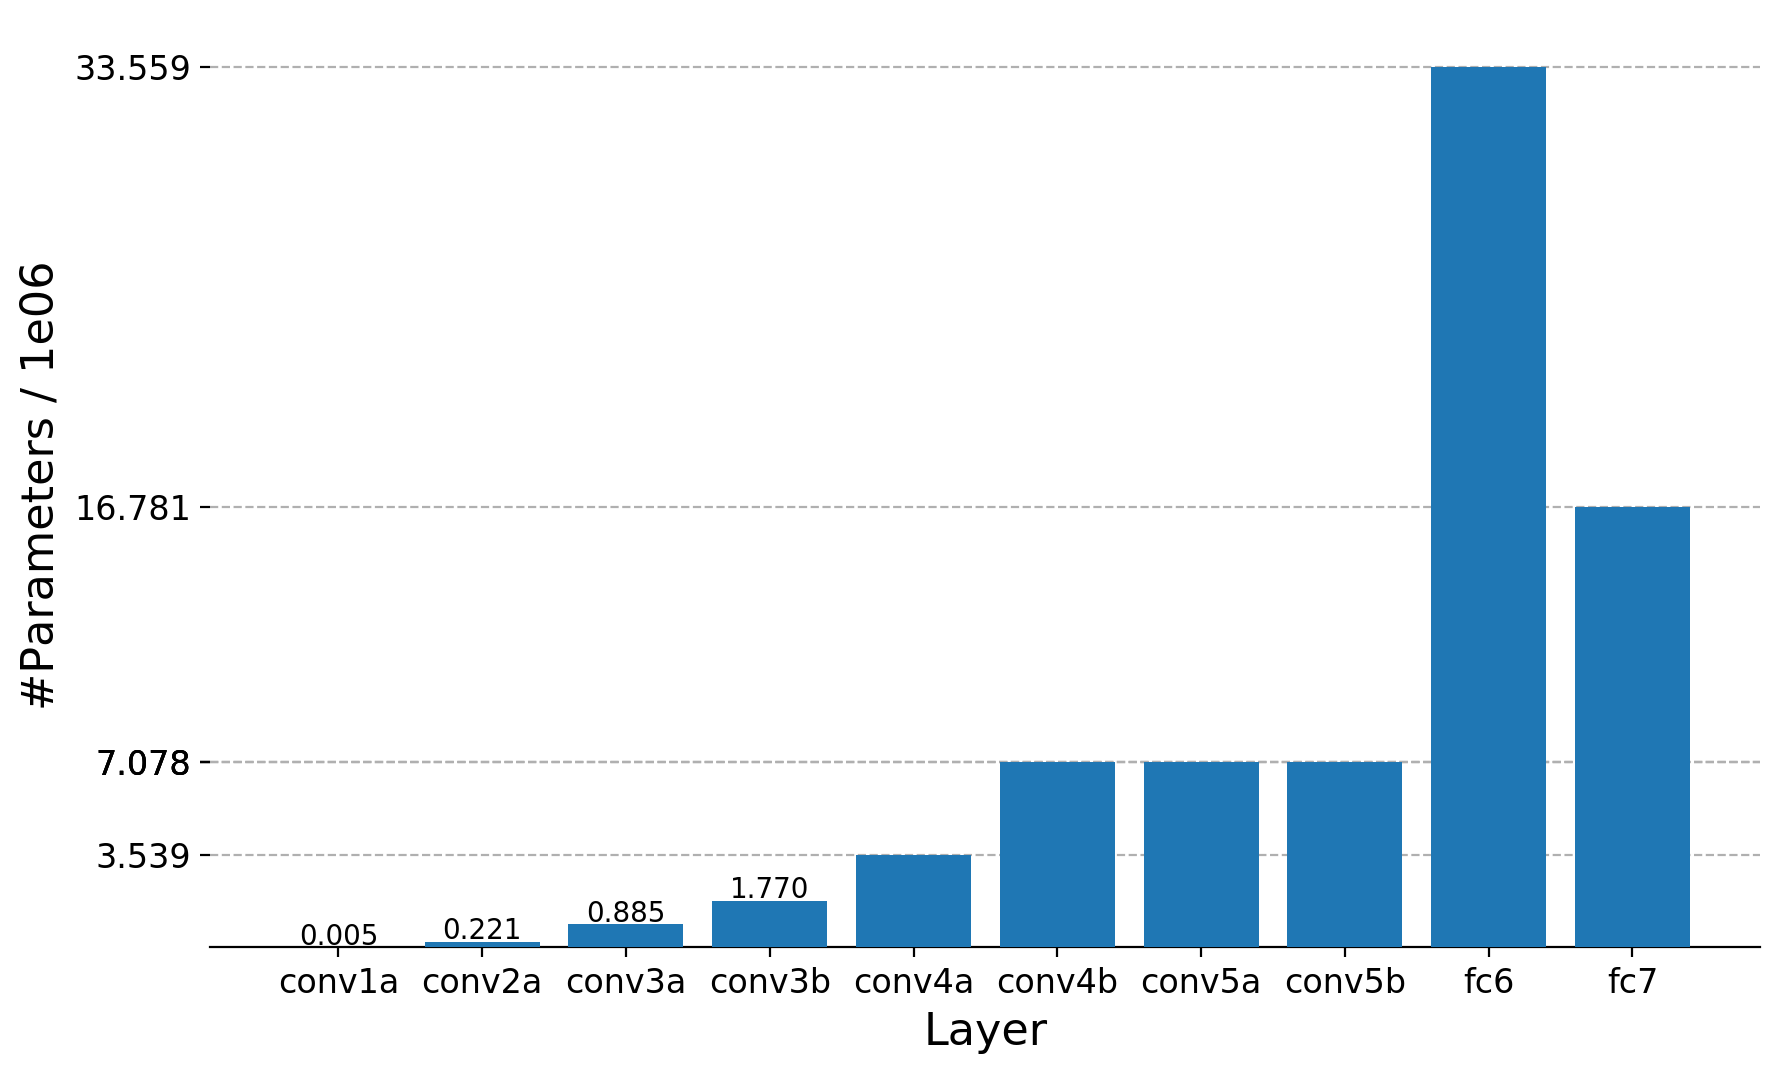
\includegraphics[width=\textwidth]{img_approach/parameters_plot}
    \caption{Distribution of parameters in our implementation of the \textit{C3D} model. Parameters in the last softmax layer are not included, because they depend on the number of output-classes in the target dataset.}
    \label{fig:parameters_plot}
\end{figure}

\subsubsection{Regularization Methods}
Dropout

L2 Regularization

No Batch Normalization.

Data augmentation (see \dots)

\subsection{Input Pipeline}

A single network training step in our multi-GPU setup, i.e. processing an input batch and updating the model parameters as described in section \ref{sec:multi_gpu}, takes longer than preparing a single input batch.

This is due to the following reasons:
\begin{itemize}
    \item 
    Common sizes of action recognition video-datasets make it impossible to completely keep them in main memory.
    Therefore source videos need to be loaded from slower mass storage, in order to be processed further.
    \item 
    Videos are encoded to reduce their file-size and need to be decoded to obtain the frame-by-frame RGB-values.
    Pre-decoding would heavily increase the dataset size and exceed the storage limit of our hardware.
    \item
    Source videos usually have a higher spatial resolution than necessary as network input and need to be rescaled.
    \item
    It is common practise to perform data-augmentation, i.e. to artificially increase the number of unambiguous network inputs by manipulating the source data, usually through cropping, flipping or rescaling.
\end{itemize}

Therefore, even if the input-batch generation and model training would run in parallel in two different threads, the GPUs would not receive enough data to fully unlock the potential training speed-up of a multi-GPU setup.
To mitigate this problem, we implement a multi-threaded input pipeline, which can easily be scaled to more powerful CPUs (more processing cores) and is illustrated in figure \ref{fig:input_pipeline}.

\begin{figure}[H]
    \centering
    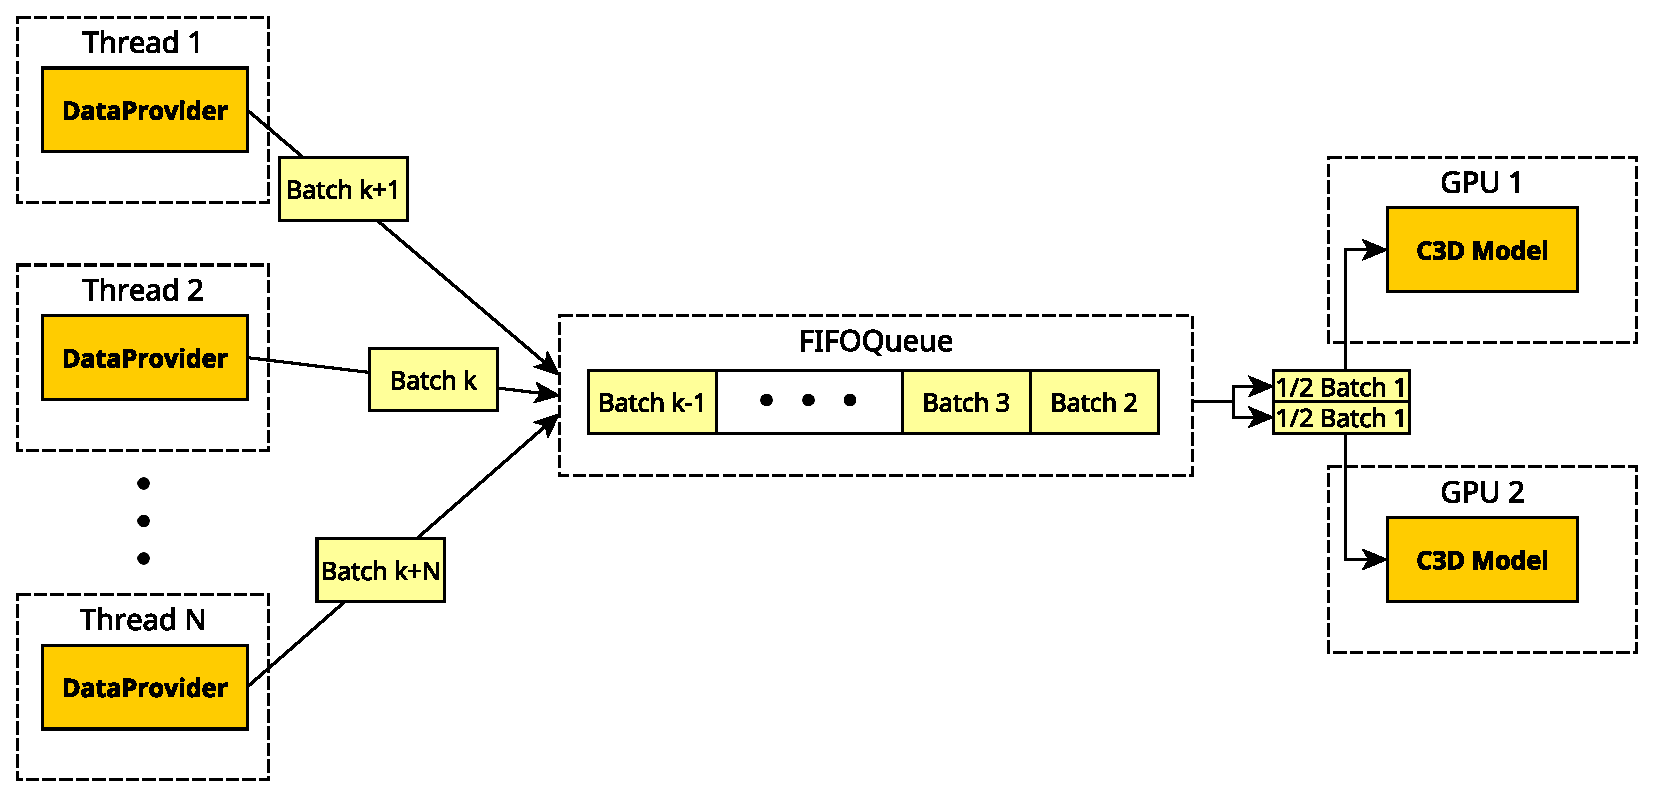
\includegraphics[width=\textwidth]{img_approach/input_pipeline.eps}
    \caption{Illustration of the multi-threaded input pipeline. A \texttt{DataProvider} instance prepares input batches in parallel to provide enough data for the GPUs. Finished batches are enqueued asynchronously into a FIFO queue which then feeds the GPUs. Batches contain input video clips as well as training labels.}
    \label{fig:input_pipeline}
\end{figure}

An arbitrary number of threads can be created to asynchronically preprocess input batches.
The maximum reasonable number of threads depends on the number of CPU cores available on the target hardware.
Each thread has a reference to a single \texttt{DataProvider} instance, which encapsulates and provides the necessary pre-processing operations to produce an input batch in a single method (\texttt{get\_next\_training\_batch()}).
This method accesses a thread-lock to ensure synchronization between the threads, i.e. no thread will pre-process the same video during an epoch\footnote{An epoch describes a complete iteration through the training set.}.
As soon as the end of an epoch is reached, that is when one thread encounters the end of the training set, all other threads wait until the last batch is processed.
The training set is then randomly shuffled and the next epoch begins.

The batches get enqueued into a single FIFOQueue which resides in the main memory.
An input batch is then dequeued from the queue whenever necessary, i.e. after the previous training step completed on the GPUs.
Several kinds of queues as well as appropriate mechanisms to asynchronically enqueue and dequeue data are supported in the \textit{Tensorflow} framework \cite{abadi_tensorflow:_2016}.

The FIFOQueue represents as a buffer between the mass storage and the data-processing GPUs.
The currently enqueued number of batches thereby provides an accurate measure of the data flow, i.e. if more than one batch is enqueued during the overall training process, then the GPUs never had to wait for data.
Only in this case does the training process fully benefit from a multi-GPU setup.


\subsection{Multi-GPU Stochastic Gradient Descent}
\label{sec:multi_gpu}

Stochastic gradient descent.

Incorporating multiple GPUs for parallel training of a deep neural network is not a trivial task and there are different ways to do so.
Parallelising network training with multiple GPUs can be divided into the following main approaches:
\begin{enumerate}
    \item Model Parallelism
    \item Data Parallelism
    \begin{enumerate}
        \item Asynchronous model updates
        \item Synchronous model updates
    \end{enumerate}
\end{enumerate}

\subsubsection{Model Parallelism}
Model parallelism describes dividing the to be trained network model into multiple parts and calculating each of these parts on a separate device.
Parallelizing a neural network that way turns out to be difficult, since the model needs to be split in a way to reduce cross-GPU communication as much as possible.
Particularly in fully-connected networks, splitting the model results in a lot of cross-device communication and generally no speed-up can be obtained from this approach.
The advantage of model parallelism therefore heavily depends on the network architecture itself.
Convolutional neural networks contain locally connected patches of neurons and are therefore easies to split, i.e. with less resulting cross-device communication.

The most intuitive way of splitting a network model horizontally, results in no parallelization speed-up at all, because the layers on GPU $n$ always have to wait for the outputs of GPU $n-1$.

Figure \ref{fig:model_parallelism} illustrates the above discussed alternatives to parallelize a single neural network model.

\begin{figure}[H]
    \begin{subfigure}[c]{\textwidth}
        \centering
        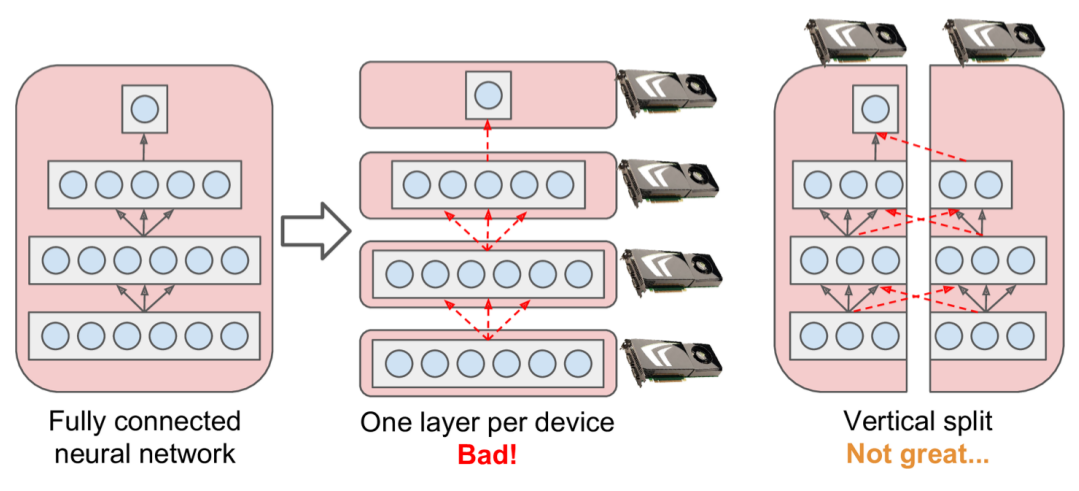
\includegraphics[height=5cm]{img_approach/model_parallelism1}
        \subcaption{Splitting a fully-connected network either layer-wise (\textit{middle}) or vertically (\textit{right}).}
        \vspace{0.5cm}
    \end{subfigure}
    \begin{subfigure}[c]{\textwidth}
        \centering
        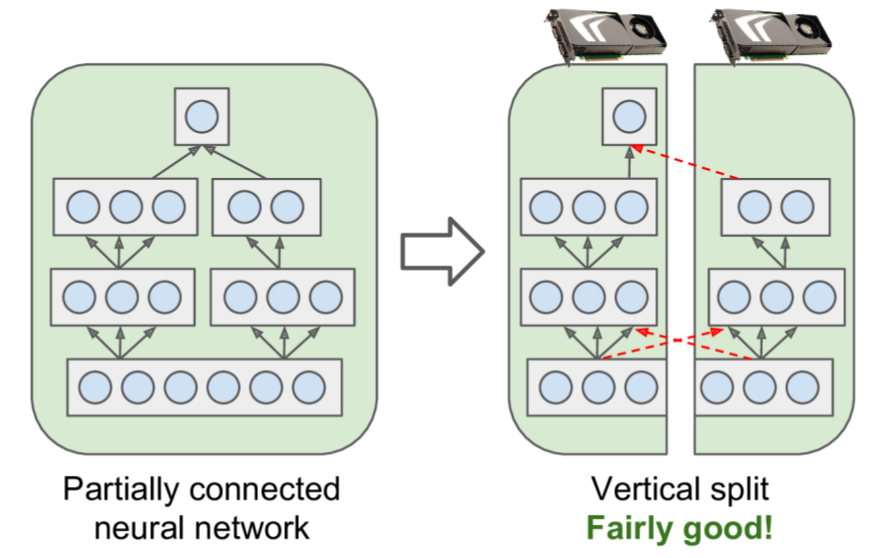
\includegraphics[height=5cm]{img_approach/model_parallelism2}
        \subcaption{Splitting a partially-connected network vertically.} 
    \end{subfigure}
    \caption{Different configurations to parallelize a single neural network model across multiple GPUs \cite{geron_hands-machine_2017}}
    \label{fig:model_parallelism}
\end{figure}

\subsubsection{Data Parallelism}
Another way to use multiple GPUs for network training is to split the input batch rather than the network model, and process these sub-batches by replicated network models across multiple GPUs in parallel.
This approach is called data parallelism and each available GPU hosts an exact replica of the model that is to be trained.
An additional set of model weights is kept in the main memory to provide synchronization for the models before each new training step.
Figure \ref{fig:data_parallelism} provides an illustration of data parallelism in a multi-GPU setup.

\begin{figure}[H]
    \centering
    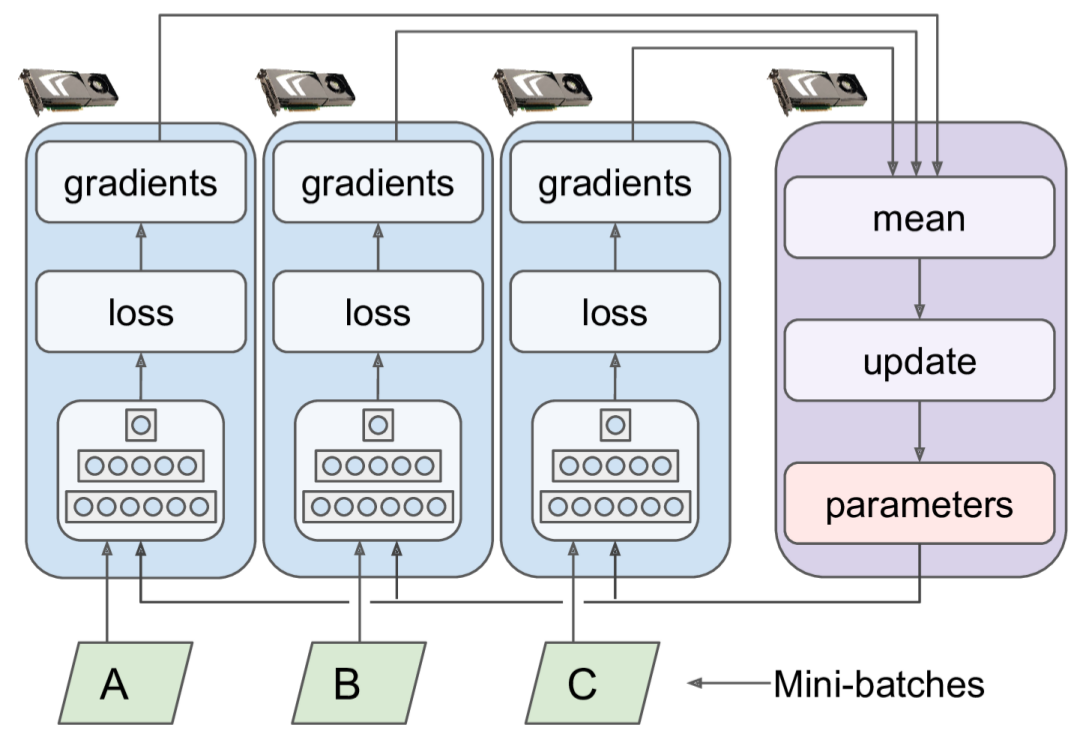
\includegraphics[width=0.7\textwidth]{img_approach/data_parallelism}
    \caption{General overview of multi-GPU training with data parallelism. \cite{geron_hands-machine_2017}}
    \label{fig:data_parallelism}
\end{figure}

Data parallelism hence yields additional computational overhead, because the shared model weights in the main memory need to be updated.
Since each model processes a sub-batch individually on its host GPUs, each model also calculates an individual set of weight updates, which needs to be communicated and merged with the weights in the main memory.
Since each GPU only processes a smaller sub-batch, the initial batch size can be increased.
This can be done in two ways: \textit{synchronically} or \textit{asynchronically}.

When updating the shared model weights \textit{synchronically}, the averaging step waits for all GPUs to finish the calculation of their individual gradients.
The averaged weight updates are then applied to the shared model weights, which are afterwards communicated back to the GPUs and thus synchronize the models to a homogeneous weight-state.
The models then proceed to process the next set of sub-batches.

Synchronous weight updates have the disadvantage, that the overall weight update has to wait for the slowest GPU to finish its computation.

Another option is to perform \textit{asynchronous} updates of the shared model parameters.
In that case, the gradients of a model are immediately used for updating as soon as a GPU finished its computation.
This averts the averaging delay and waiting for the slowest GPU.
However asynchronous updates yield the problem of ``stale'' gradients \cite{geron_hands-machine_2017}, i.e. whenever an update according to a GPU's gradients is issued, the shared weight may have been updated in the meantime and the current updates may not be beneficial anymore.

Benchmarking experiments conducted by Google Brain \cite{chen_revisiting_2016} indicate, that data parallelism with synchronous weight updates performs best.
Since our \textit{C3D} model contains locally connected convolutional layers as well as large fully-connected layers, it is difficult to split, i.e. to incorporate model parallelism for training.
Additionally, video-inputs are naturally bigger than images.
Since the amount of available memory on the GPUs limits the size of the input batches, training with data-parallelism is tempting.
We therefore decide to perform data parallel stochastic gradient descent.

\begin{figure}[H]
    \centering
    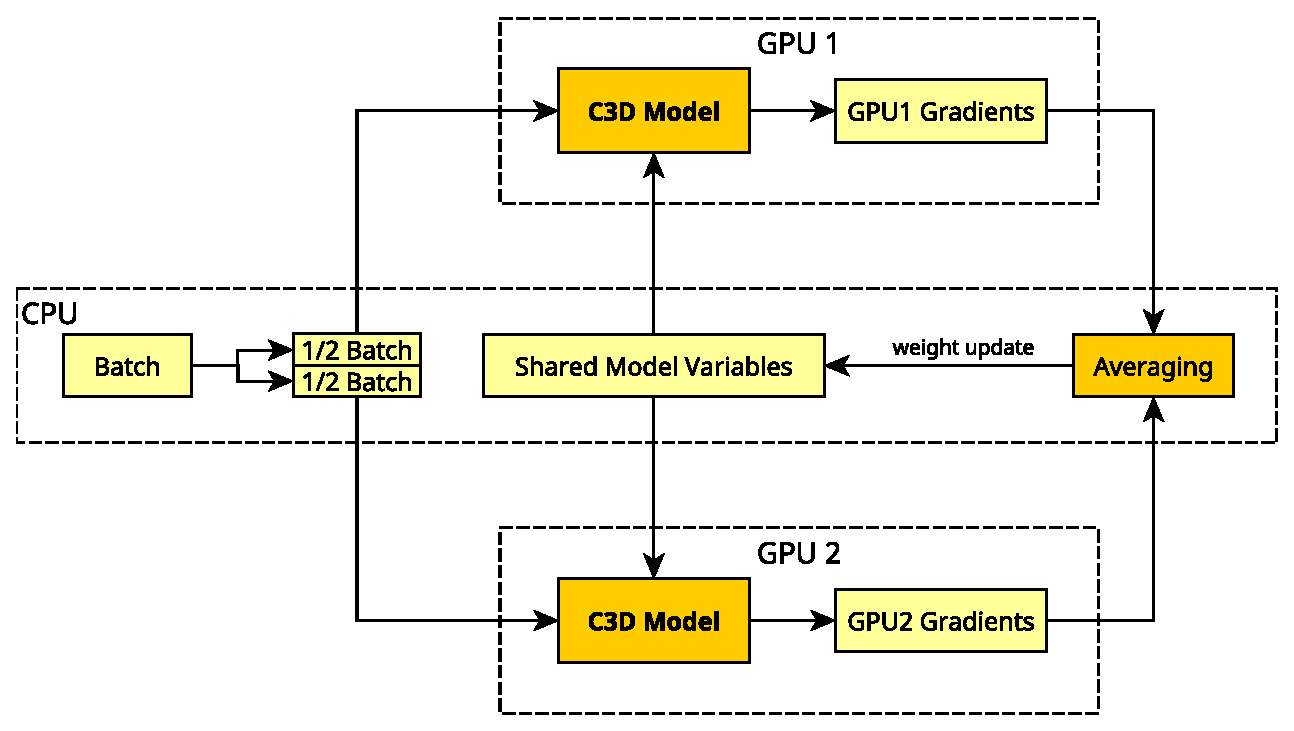
\includegraphics[width=\textwidth]{img_approach/gradient_averaging.eps}
    \caption{Diagram of a single weight update step during data parallel synchronous stochastic gradient descent.}
    \label{fig:gradient_averaging}
\end{figure}


\subsection{Input Sampling}
Our \textit{C3D} model processes input clips with a length of $16$ frames per training step, yet most source videos provide more frames, i.e. have a longer temporal duration.
A sampling strategy to provide the network with properly sized inputs ($112 \times 112 \times 16$ pixels) is therefore needed.
This primarily includes temporal cropping, that is selecting a $16$ frame long sub-clip from the full temporal evolution of the video.
We additionally incorporate spatial cropping: Source videos are initially rescaled to a larger spatial resolution and frames with the necessary width and height are then cropped out to produce network inputs.

\subsubsection{UCF-101 Input-Clips}
All source videos in the UCF-101 dataset are provided in a fixed resolution of $320 \times 240$ pixels (width $\times$ height) with an average length of $7.21s$ \cite{soomro_ucf101:_2012}.
Video in the training- as well as test-set of UCF-101 are annotated with a single action label.
During training we iterate over the list of training videos and sample one input clip for each of those training-videos.
The number of finished training epochs therefore corresponds to the overall number of processed input-clips per source video.

To reduce pre-processing time per training step, only a $16$ frame long time-interval is decoded from the source training video.
For UCF-101 training, this interval is randomly sampled from the complete training video, since it only contains one single action.
The resulting $16$ frames are then rescaled to a fixed spatial resolution of $160 \times 120$ pixels.
The final network input is then cropped out by randomly selecting a $112 \times 112$ pixels wide region in the first frame and cropping the 15 following frames accordingly.

Following this procedure a multitude of network inputs can be sampled from a single source video.
We use a batch size of $40$ per training step, which results in $20$ clips per GPU during training.
This was found to be the biggest possible number of inputs to not exceed memory limitations of the available GPUs.

\subsubsection{Charades Input-Clips}
The source videos in the Charades dataset are provided in multiple resolutions.
To reduce the download time and dataset size, the $480p$-version of the dataset was downloaded, which contains videos with a maximal height of $480$ pixels.
In contrast to UCF-101 a single source video is annotated with multiple action instances, which can possibly overlap.
To fit training on the Charades dataset in our implemented pre-processing pipeline, we treat each annotated action instance as a single source video, from which input-clips can be sampled.

During training on the Charades dataset we iterate over the list of temporally localized action instances and again sample one network input-clip per instance.
To reduce pre-processing time, only a $16$ frame long interval is decoded from each action instance in the training set.
Analogously to the input sampling procedure on UCF-101 this interval is selected randomly.
Since the videos have different spatial resolutions, we rescale the shorter side of previously sampled interval to $120$ pixels and 
spatially crop consecutive $112 \times 112$ pixel wide regions.

Training on the Charades does not influence the batch-size, which is therefore kept at 40 input clips per batch.

\subsubsection{3D Temporal Order Verification}
Since obtaining the labels \textit{correct temporal order} and \textit{incorrect temporal order} is practically free (see \ref{subsec:tov}), \textit{temporal order verification} can be seen as an unsupervised pre-training method.
Therefore also a large amount of unlabelled data can be used in the pre-training process, as long it contains videos of (preferably human) motion.

Promising candidate datasets are ActivityNet, because it contains a bib number of weakly annotated and non-localised human activities as well as Kinetics, which provides a big number of temporally localized actions.
These datasets however are only distributed via YouTube, i.e. each video needs to be downloaded individually.
At the time of this writing about half of the training-set of Kinetics could be obtained.
To provide a closed basis for evaluation of our approach, experiments were limited to sampling \textit{temporal order verification} tuples from the source datasets themselves, i.e. UCF-101 and Charades.

Successful pre-training with \textit{temporal order verification} requires providing inputs, which are distinguishable when permuted randomly, as described by \textcite{misra_shuffle_2016}.
This means in practise for our \textit{C3D} model, that a sampled input clip needs to contain a certain amount of motion, in order to be beneficial for pre-training.
A video clip with a small magnitude of motion looks nearly the same, when permuted.


